\section{ML Model Results}\label{sec:results_ML}
In this section we present the results of the ML models we have trained. We then deeply inspect the best performing model,
in order to understand its features and its performance.


% --------------- Model Selection ---------------

\subsection{Model Selection}\label{subsec:results_ML_model_selection}
As previously shown by the operative flow in Figure~\ref{fig:ML_operative_flow}, there are several phases involved in the
selection of the optimal prediction model. Given our limited resources we chose to take a greedy approach by performing
the feature selection first, and then optimizing the hyperparameters at a later time for each of the three models considered.
% MATTEO
% - Matrix plot of stepwise (which is results of algorithm 1) for each model --> to justify the chosen features
\subsubsection*{Features Selection}
To reduce the amount of time spent training the models to select the best hyperparameters, it is best to first limit the
number of features considered. The selection of the most useful features was performed using a forward stepwise selection,
following a greedy a approach that aims at maximizing the accuracy. The hyperparameters were initalized with the default
values provided by the library scikit-learn.\\
As depicted in Figure~\ref{fig:stepwise_acc_logreg}, we can see that the best accuracy with the logistic regression
model is reached after the third iteration, with little improvement with respect to the model using a single feature.
This kind of model seems to favor information about communities and the L2 measure. The feature about the community count is weak on its own,
being the only one that adds 3 columns, but it seems to carry complementary information with respect to the other features,
raising the accuracy by a small margin.
\begin{figure}[h]
	\centering
	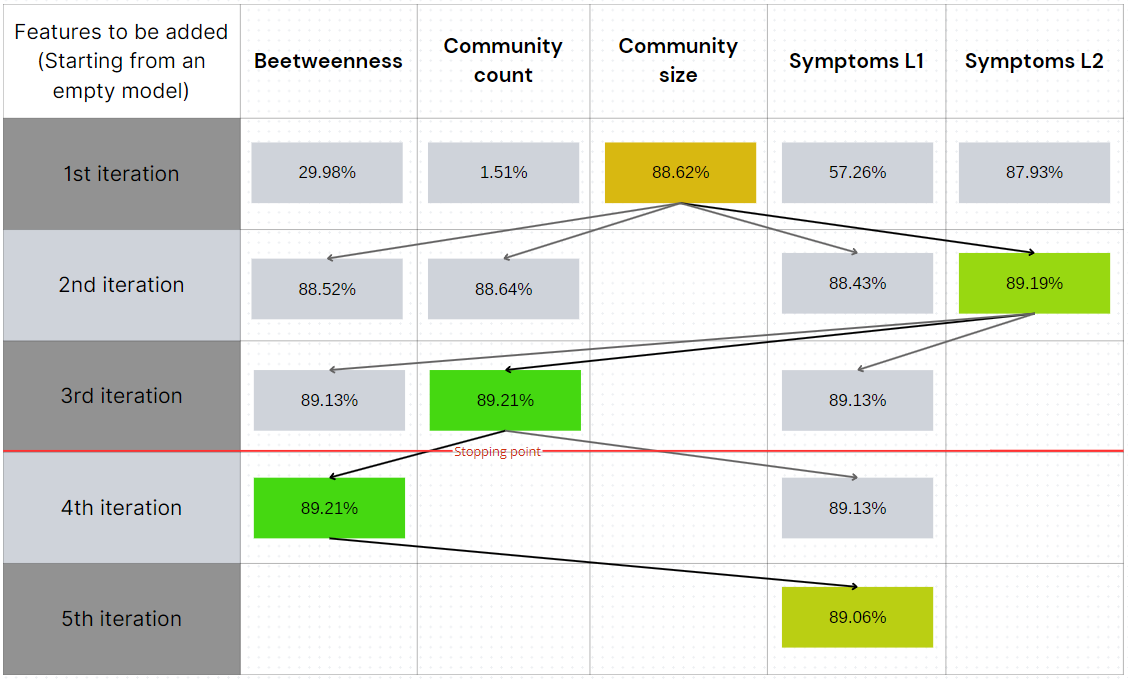
\includegraphics[width=\columnwidth]{stepwise_acc_logreg.png}
	\caption{Accuracy of the logistic regression models over the iterations of the forward stepwise feature selection}\label{fig:stepwise_acc_logreg}
\end{figure}
\noindent
Figure~\ref{fig:stepwise_acc_randomforest} shows that the random forest models work best with less information than logistic regression.
In this case the only features retained are the ones about communities: these results start to reveal which features are the most useful
when it comes to classification.
It is also worth noting that the best random forest model has a slightly worse accuracy than logistic regression,
but that might be due to the random choice of the model's parameters.

\begin{figure}[h]
	\centering
	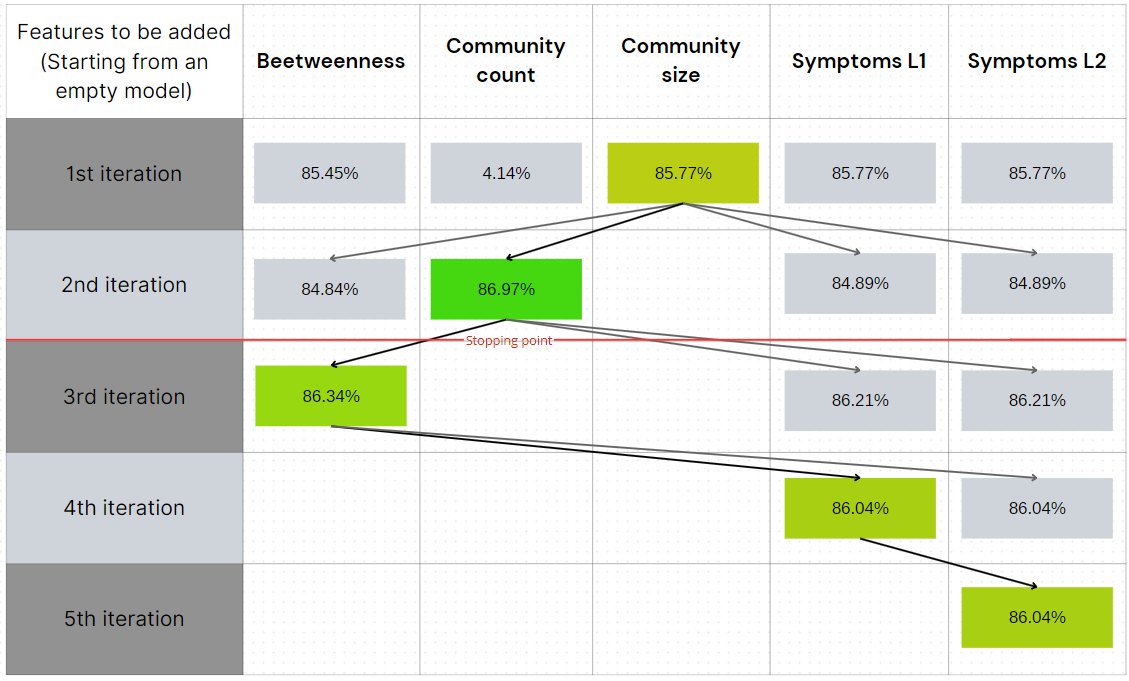
\includegraphics[width=\columnwidth]{stepwise_acc_randomforest.png}
	\caption{Accuracy of the random forest models over the iterations of the stepwise feature selection}\label{fig:stepwise_acc_randomforest}
\end{figure}
\noindent
The multi-layer perceptron model stands in the middle with respect to the other two models in terms of accuracy.
As underlined by Figure~\ref{fig:stepwise_acc_mlp}, unlike the other two cases the model performs its prediction by leveraging only the L2 features,
enhanced by the smaller community count. Two steps are enough to reach the best possible test accuracy.
This particular implementation of neural network has one hidden layer with 100 neurons, and in our case its performance is better
than the random forest model, but still slightly worse than the logistic regression. We expect this to change after the optimization of the hyperparameters,
due to the ability of the MLP to `see' non-linearities.

\begin{figure}[h]
	\centering
	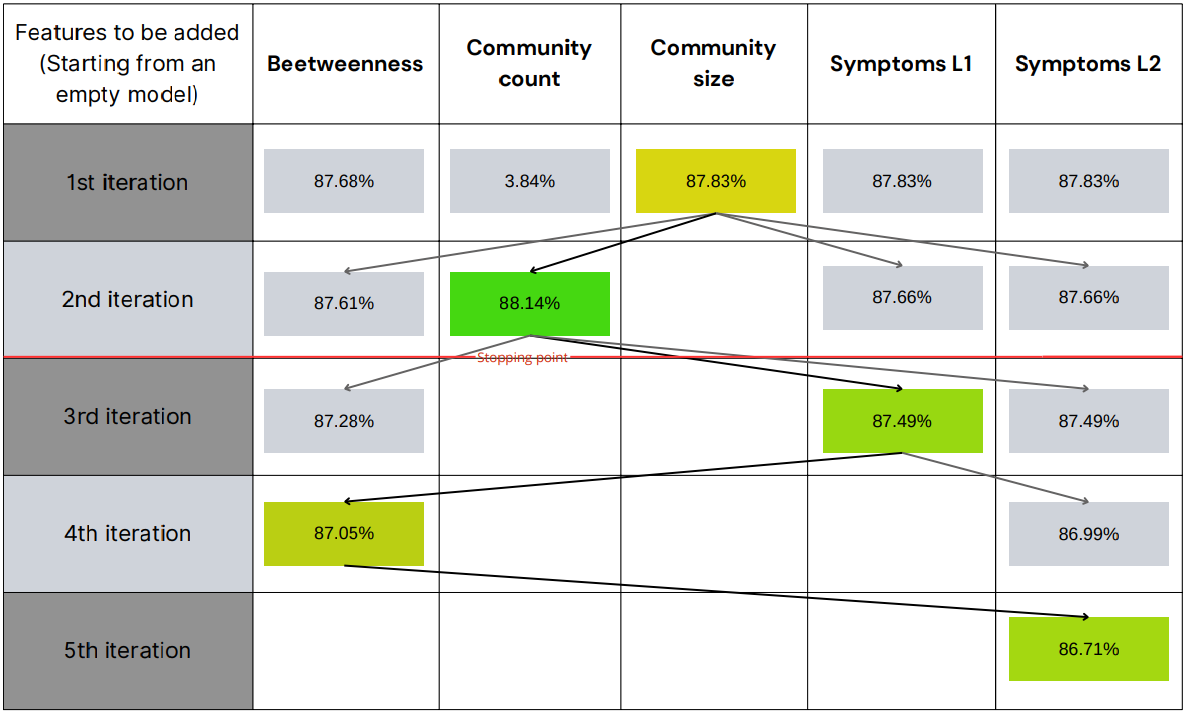
\includegraphics[width=\columnwidth]{stepwise_acc_mlp.png}
	\caption{Accuracy of the MLP models over the iterations of the stepwise feature selection}\label{fig:stepwise_acc_mlp}
\end{figure}

\nocite{Zhang_2016}
% CRISTIAN
% - Comparison for each model of the selected parameters --> to justify the chosen parameters
\subsubsection*{Hyperparameters Selection}

The process of hyperparameter tuning was integral to optimizing the performance of our machine learning models.
We experimented with a range of hyperparameters for each model and identified the best configurations based on test accuracy.
Tables~\ref{logistic_regression_hyperparams},~\ref{random_forest_hyperparams}, and~\ref{mlp_hyperparams} detail the hyperparameters
tested and the best selections for Logistic Regression, Random Forest, and Multi-Layer Perceptron (MLP) respectively.

\rowcolors{2}{blue!8}{blue!18}
\begin{table}[h]
	\centering
	\small
	\begin{tabular}{|c|c|c|}
		\hline
		\textbf{Hyperparameters} & \textbf{Test}                                                                                   & \textbf{Best}                                               \\
		\hline
		C                        & \begin{tabular}[c]{@{}c@{}}0.001, 0.01, 0.1, 0.5,\\ 0.75, 1, 1.25,\\ 1.50, 10, 100\end{tabular} & 1.5                                                         \\
		max iter                 & \begin{tabular}[c]{@{}c@{}}100, 200, 300,\\ 500, 1000\end{tabular}                              & \begin{tabular}[c]{@{}c@{}}Until\\ Convergence\end{tabular} \\
		penalty                  & \begin{tabular}[c]{@{}c@{}}l1, l2,\\ None\end{tabular}                                          & l2                                                          \\
		solver                   & \begin{tabular}[c]{@{}c@{}}lbfgs,\\ liblinear,\\ newton-cg\end{tabular}                         & lbfgs                                                       \\
		\hline
	\end{tabular}
	\caption{Best Hyperparameters for Logistic Regression}
	\label{logistic_regression_hyperparams}
\end{table}

\rowcolors{2}{blue!8}{blue!18}
\begin{table}[h]
	\centering
	\small
	\begin{tabular}{|c|c|c|}
		\hline
		\textbf{Hyperparameters} & \textbf{Test}                                                                    & \textbf{Best} \\
		\hline
		n estimators             & \begin{tabular}[c]{@{}c@{}}50, 80, 100,\\ 200, 300, 400,\\ 500, 600\end{tabular} & 600           \\
		max depth                & \begin{tabular}[c]{@{}c@{}}25, 50, 60,\\ 75, 100, None\end{tabular}              & 50            \\
		min samples split        & \begin{tabular}[c]{@{}c@{}}2, 5,\\ 10, 20\end{tabular}                           & 2             \\
		min samples leaf         & \begin{tabular}[c]{@{}c@{}}1, 2,\\ 5, 10\end{tabular}                            & 1             \\
		\hline
	\end{tabular}
	\caption{Best Hyperparameters for Random Forest}
	\label{random_forest_hyperparams}
\end{table}

\rowcolors{2}{blue!8}{blue!18}
\begin{table}[h]
	\centering
	\small
	\begin{tabular}{|c|c|c|}
		\hline
		\textbf{Hyperparameters} & \textbf{Test}                                                                                                                                                  & \textbf{Best}     \\
		\hline
		First hidden layer       & \begin{tabular}[c]{@{}c@{}} (300)\\ (400)\\(100, 50)\\(500, 200)\\ (60), (80)\\(100), (200)\\ (100, 100, 100)\\ (900, 800, 700)\\ (700, 300, 100)\end{tabular} & (80)              \\
		max iter                 & \begin{tabular}[c]{@{}c@{}}100, 200\\ 300, 500\\ 1000\end{tabular}                                                                                             & Until Convergence \\
		alpha                    & \begin{tabular}[c]{@{}c@{}}0.0001, 0.001\\ 0.01, 0.1, 1\end{tabular}                                                                                           & 0.0001            \\
		activation               & \begin{tabular}[c]{@{}c@{}}relu, tanh\\ logistic, identity\end{tabular}                                                                                        & relu              \\
		\hline
	\end{tabular}
	\caption{Best Hyperparameters for MLP}
	\label{mlp_hyperparams}
\end{table}
\noindent
These hyperparameter configurations were carefully selected to maximize the performance of each model. The Logistic Regression model, with its optimal C value and penalty type, demonstrates a balance between model complexity and regularization. The Random Forest model's parameters, such as the number of estimators and maximum depth, were chosen to balance the bias-variance trade-off, ensuring robustness and generalization. Lastly, the MLP model, with its specific hidden layer sizes and activation function, was configured to effectively capture complex, non-linear relationships in the data.


% ANDREA
% - Comparison of the three models with best combination of features and best parameters
% - precision, recall, AUC, accuracy
\subsubsection*{Model Comparison}\label{subsubsec:results_ML_model_comparison}

As illustrated in Figure~\ref{fig:ML_operative_flow}, our model ensemble now comprises six variants:
three leveraging only symptoms and three incorporating new network-based features. The selection of
the best-performing model from each group was based on test accuracy assessment, where the test is the same balanced dataset
in all cases. Figure~\ref{fig:acc_symptoms}
illustrates consistently low overfitting across all models, showcasing the stability of the symptom-only
models. In contrast, Figure~\ref{fig:acc_new_features}, portraying the accuracy of models with the new
features, reveals some overfitting, particularly in the MLP and Random Forest.\\
The observed tendency for models with new features to exhibit more pronounced overfitting is unsurprising,
given the greater number and complexity of these features compared to symptoms. Notably, despite their different
complexity, all models demonstrate similar test accuracy levels, suggesting that a linear separation
boundary suffices for effective feature classification. Considering this, we retain the Logistic Regression
model as the best-performing model in each group, striking a balance between performance and complexity.

\begin{figure}[h]
	\centering
	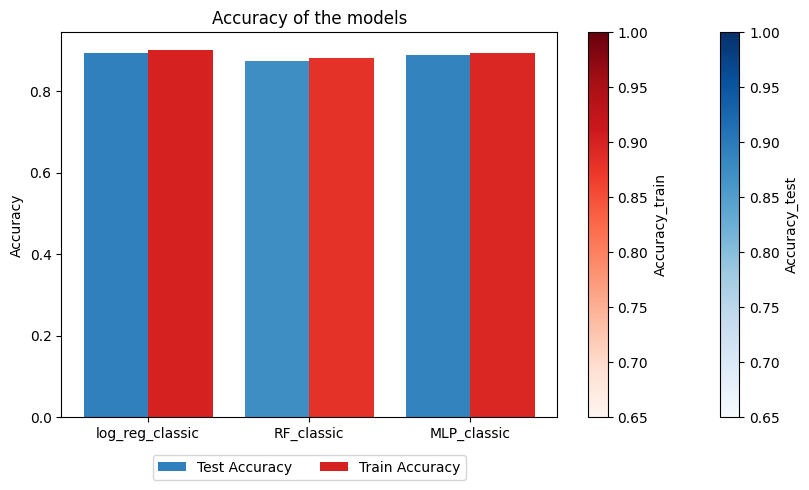
\includegraphics[width=\columnwidth]{acc_symptoms.png}
	\caption{Accuracy of the three models with only symptoms}\label{fig:acc_symptoms}
\end{figure}

\begin{figure}[h]
	\centering
	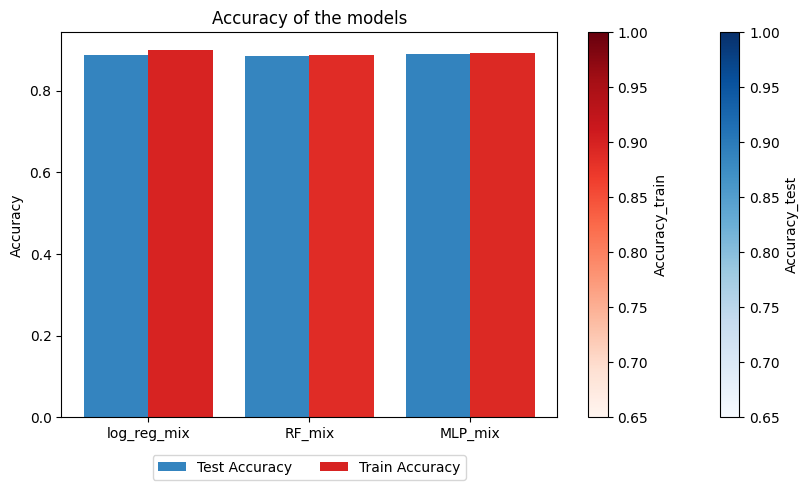
\includegraphics[width=\columnwidth]{acc_new_features.png}
	\caption{Accuracy of the three models with new features}\label{fig:acc_new_features}
\end{figure}



% --------------- New Features Effect ---------------

\subsection{New Features Effect}
% ANDREA
% - compare the best symptoms one hot model with the best one with the new features

\noindent
The best model from each group was further trained on the full balanced dataset to ensure a more reliable
performance evaluation and the test accuracy was computed on the real unbalanced data.
The results in Figure~\ref{fig:acc_best_models} reveal a minimal difference between
the two groups. This addresses our \textbf{first goal}: the new features, only slightly improve the model,
offering a comparable performance to using symptoms alone. However, It's essential to note that the new features are
more numerous than the symptoms, contributing to a more complex model. In conclusion, the extracted network
features are not a superior alternative to symptoms.\\
It is worth to underline that the `simplicity' of the dataset, which leads to a very high accuracy in all models, may also affect the performance
evaluation of the new features, which have a small room to improve the model. Therefore, a possible avenue
for future exploration could involve the use of more complex dataset, to better assess the performance of the
new features.\\
Another viable option for future work is to use the new features as a complement to the symptoms.


% THE FIGURE IS THE FIGURE OF MODEL FULLY TRAINED ON THE BALANCED DATASET


\begin{figure}[h]
	\centering
	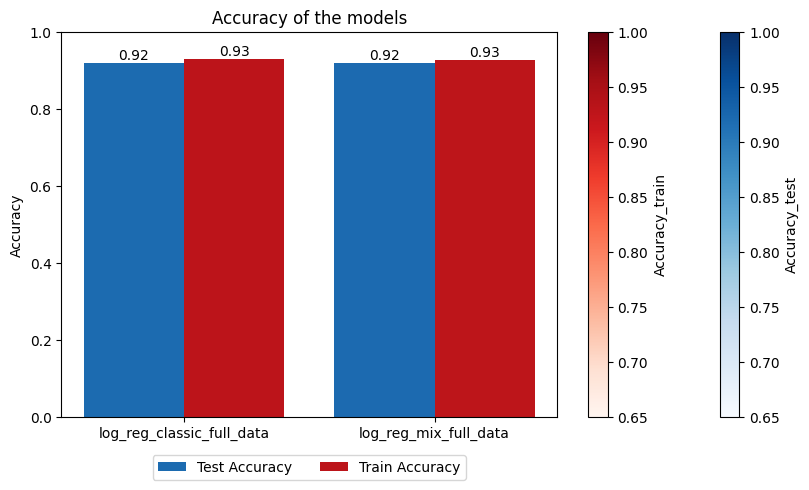
\includegraphics[width=\columnwidth]{acc_best_models.png}
	\caption{Accuracy of the best models from both groups}\label{fig:acc_best_models}
\end{figure}



% --------------- Best Model Performance ---------------

\subsection{Best Model Analysis}
Given that the logistic regression using only symptoms and the one with the new features achieve the same accuracy,
we have selected the logistic regression with the new features as the superior model for further analysis.
Considering its greater complexity and the small level of overfitting,
this model has the potential to capture more nuanced information and intricate patterns.\\
The model contains 3 group of features: community size, SI index level 2 and community count.
\subsubsection*{Performance analysis}
The performance of our predictive model, as demonstrated by the confusion matrix in Figure \ref{fig:conf_matrix},
is indicative of its capability to effectively distinguish between different disease classes.
These classes are stratified based on their respective Disease Influence (DI) indices.

\begin{itemize}
	\item \textbf{Class 1: Low DI L1 - Low DI L2:} Diseases with a low degree (DI L1) and limited connections to other symptoms (DI L2)
	      tend to be highly specific, which is reflected in the model's precision for such cases.
	      The confusion matrix exhibits a low misclassification rate for these diseases,
	      suggesting that when such specific symptoms are presented, the model can predict with high confidence,
	      albeit for a restricted number of cases.

	\item \textbf{Class 2: Low DI L1 - High DI L2:} Diseases characterized by a low DI L1 but a high DI L2 are connected to a few symptoms,
	      which in turn are associated with a wider array of other diseases. The model's performance for these diseases,
	      as shown in the confusion matrix, presents a moderate degree of accuracy.
	      Misclassifications may occur due to the broader symptom overlap with other diseases.

	\item \textbf{Class 3: High DI L1 - Low DI L2:} A high DI L1 coupled with a low DI L2 signifies diseases with numerous related symptoms,
	      which however, do not significantly influence other diseases.
	      The confusion matrix suggests that such diseases are predicted with a considerable degree of accuracy.
	      The symptoms, while not disease-specific, contribute to a heightened overall model performance due to their prevalence.

	\item \textbf{Class 4: High DI L1 - High DI L2:} Diseases with both high DI L1 and DI L2 indices are those that exhibit common symptoms
	      influencing a multitude of other diseases. The confusion matrix shows that the model is generally accurate in predicting these diseases.
	      However, due to the commonality of symptoms, there is an inherent challenge in precisely classifying them,
	      which could result in a higher misclassification rate with diseases sharing similar symptom profiles.
\end{itemize}
\noindent
The aforementioned analysis underscores the complexity inherent in disease-symptom relationships and their impact on predictive modeling.
As the confusion matrix corroborates, our model adeptly handles diseases with distinct symptom profiles (Low DI L1 - Low DI L2)
but is challenged by diseases sharing common symptoms (High DI L1 - High DI L2).
Consequently, the model's performance is a direct reflection of the nuanced interplay between disease prevalence and symptom specificity,
as encapsulated by the DI indices.
\begin{figure}[h]
	\centering
	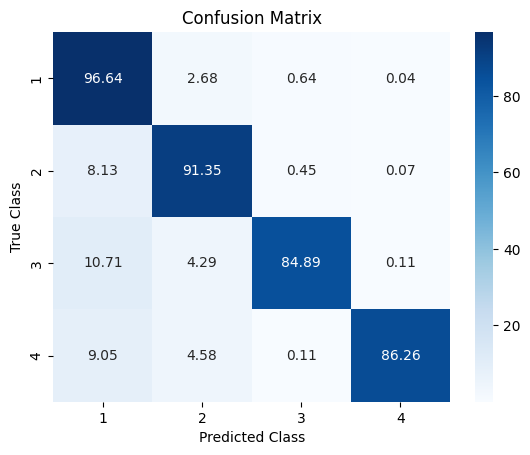
\includegraphics[width=\columnwidth]{conf_matrix_best_model.png}
	\caption{Confusion matrix of the predictive model}\label{fig:conf_matrix}
\end{figure}
\noindent
Figure~\ref{fig:performance_graph} displays a detailed comparison of the model's diagnostic efficacy for a wide range of diseases,
identified by their numerical codes on the x-axis.
The graph features two key metrics: the F1 score and accuracy, represented by blue and orange lines, respectively.
The accuracy line, mostly stable and high, shows the model's consistent ability to correctly detect both presence and absence of each disease.
In contrast, the F1 score line, more varied, reflects the complexity and variability in predicting disease symptoms,
illustrating the model's precision and recall for each disease. High points on the F1 score indicate optimal model performance,
with a balanced precision and recall, effectively identifying true disease cases without errors.
Low points, however, highlight areas where the model is less effective.
\begin{figure*}[htbp]
	\centering
	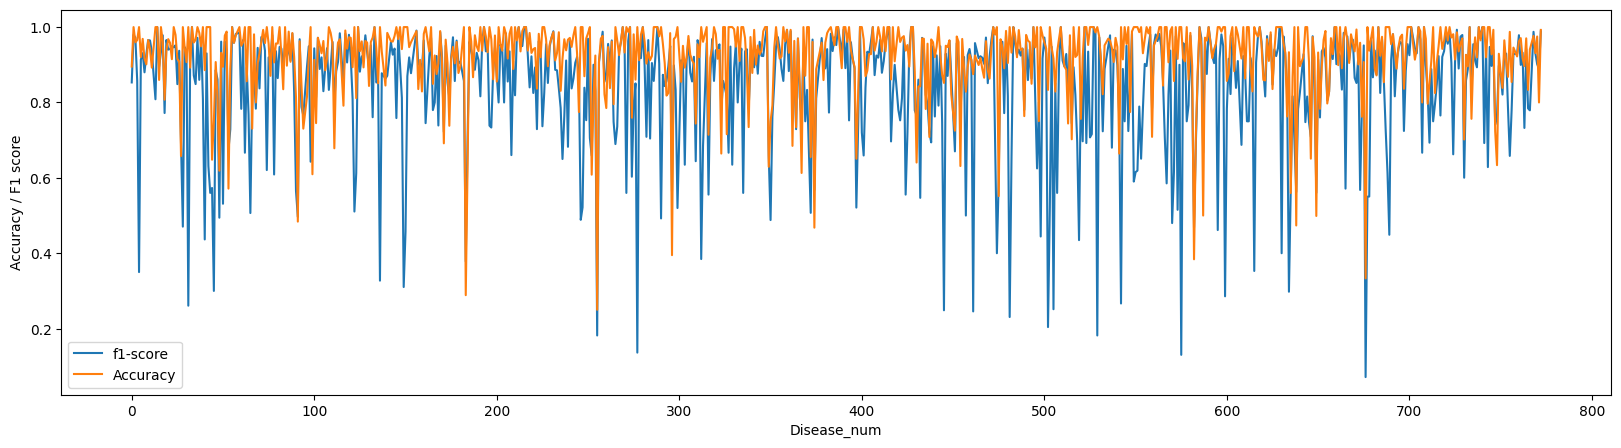
\includegraphics[width=\textwidth]{accuraci_diseases_best_model.png}
	\caption{A comparison of the F1 score and accuracy for each disease predicted by the model.}
	\label{fig:performance_graph}
\end{figure*}
\subsubsection*{Best and worst performing diseases}
Our diagnostic model's effectiveness is analyzed by assessing its performance across different diseases.\\
Table~\ref{best} lists the top ten diseases where the model demonstrates high accuracy.
This exceptional performance is further highlighted by near-perfect f1-scores, indicating an optimal balance of precision and recall.
Diseases like mitral valve disease, syndrome of inappropriate secretion, and acute bronchospasm stand out with f1-scores of 1.0,
exemplifying the model's precision in diagnosing these conditions without any errors.\\
On the other hand, Table~\ref{worst} outlines the ten diseases with the lowest accuracy,
indicating areas where the model's diagnostic efficiency is limited. While accuracy is lower for these diseases,
the f1-scores for conditions like premature ventricular contractions and histoplasmosis reveal that the model,
when accurate, maintains reasonable precision and recall.
Nevertheless, the notable decline in f1-score for ailments such as vitamin b12 deficiency and otitis media reveals a significant imbalance
in the model's diagnostic precision and recall, underscoring the need for targeted improvements in these specific areas.
\rowcolors{2}{green!8}{green!18}
\begin{table}[H]
	\centering
	\small
	\begin{tabular}{|c|c|c|}
		\hline
		\textbf{Disease}                    & \textbf{Accuracy} & \textbf{f1-score} \\
		\hline
		mitral valve disease                & 1.0               & 1.000000          \\
		syndrome of inappropriate secretion & 1.0               & 1.000000          \\
		acute bronchospasm                  & 1.0               & 1.000000          \\
		eye alignment disorder              & 1.0               & 1.000000          \\
		reactive arthritis                  & 1.0               & 1.000000          \\
		joint effusion                      & 1.0               & 0.985507          \\
		anal fistula                        & 1.0               & 0.823529          \\
		open wound of the shoulder          & 1.0               & 0.791667          \\
		alzheimer disease                   & 1.0               & 0.769231          \\
		infectious gastroenteritis          & 1.0               & 0.666667          \\
		\hline
	\end{tabular}
	\caption{Accuracy and f1 score for the 10 diseases with the highest accuracy}
	\label{best}
\end{table}


\rowcolors{2}{red!8}{red!18}
\begin{table}[H]
	\centering
	\small
	\begin{tabular}{|c|c|c|}
		\hline
		\textbf{Disease}                     & \textbf{Accuracy} & \textbf{f1-score} \\
		\hline
		premature ventricular contractions   & 0.500000          & 0.666667          \\
		histoplasmosis                       & 0.498876          & 0.560252          \\
		hemiplegia                           & 0.483908          & 0.496462          \\
		acute bronchiolitis                  & 0.473684          & 0.562500          \\
		poisoning due to antimicrobial drugs & 0.467849          & 0.567968          \\
		open wound of the mouth              & 0.394890          & 0.564315          \\
		acute otitis media                   & 0.383938          & 0.468456          \\
		vitamin b12 deficiency               & 0.333333          & 0.071429          \\
		bladder cancer                       & 0.288740          & 0.378102          \\
		otitis media                         & 0.250000          & 0.181818          \\
		\hline
	\end{tabular}
	\caption{Accuracy and f1 score for the 10 diseases with the lowest accuracy}
	\label{worst}
\end{table}

\subsubsection*{Analysis of bladder cancer}

Bladder cancer, as identified in Table~\ref{worst}, is a disease with notably low diagnostic accuracy in our model,
prompting a more detailed investigation. Figure~\ref{fig:cancer_missclassified}
illustrates the proportion of bladder cancer cases incorrectly identified by the model, revealing frequent misclassifications,
especially as diabetes insipidus and hemiplegia.\\
Figures~\ref{fig:cancer_diabet} and~\ref{fig:caner_hemiplegia} delve deeper, showing the number of bladder cancer cases exhibiting
symptoms akin to diabetes insipidus and hemiplegia, respectively. It's striking that 90\% of bladder cancer samples share
symptoms with diabetes insipidus and hemiplegia, clarifying why the model often confuses bladder cancer with these diseases.\\
Moreover, an important factor contributing to this diagnostic challenge is the representation of bladder cancer in our dataset.
Constituting only 0.36\% of the total data, this limited presence may significantly impact the model's ability to accurately identify bladder cancer,
leading to its lower accuracy for this specific condition.
\begin{figure*}[htbp]
	\centering
	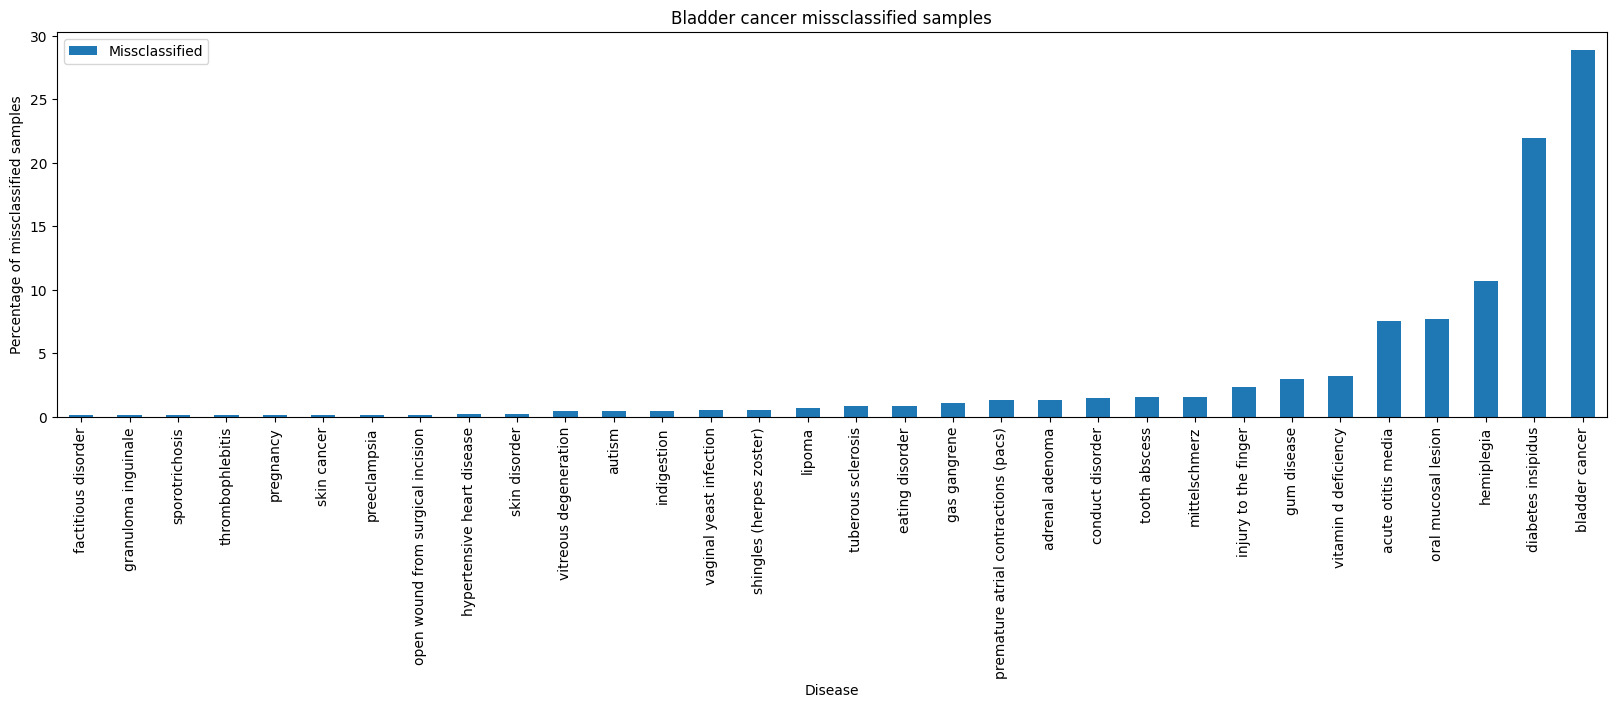
\includegraphics[width=\textwidth]{bladder_cancer_missclassified.png}
	\caption{Percentage of bladder cancer samples misclassified}\label{fig:cancer_missclassified}
\end{figure*}
\noindent

\begin{figure}[h]
	\centering
	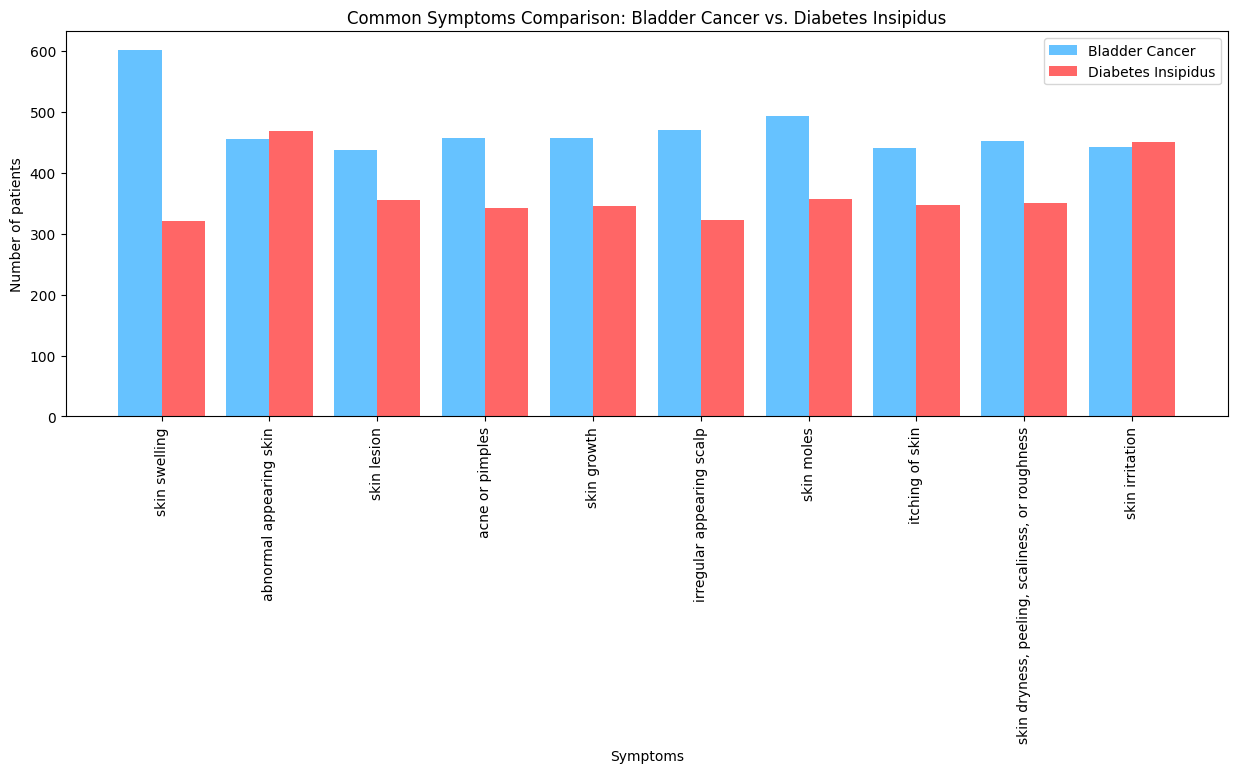
\includegraphics[width=\columnwidth]{cancer_diabet}
	\caption{number of samples of bladder cancer and diabets insipidus that have the same symptoms}\label{fig:cancer_diabet}
\end{figure}
\noindent

\begin{figure}[h]
	\centering
	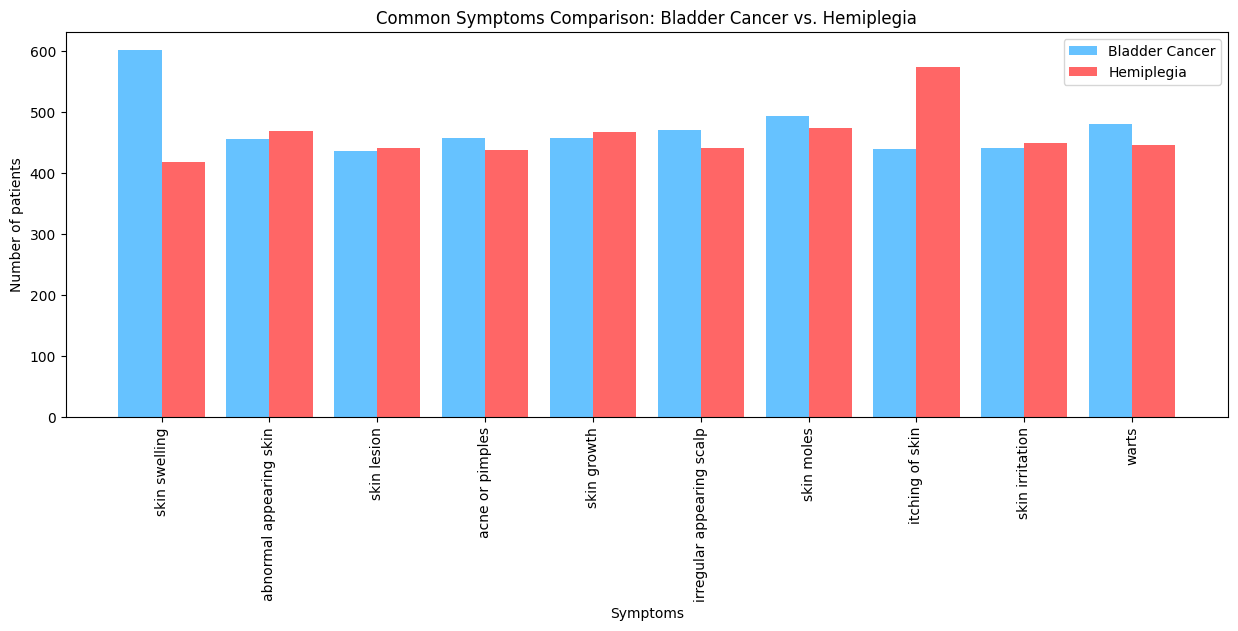
\includegraphics[width=\columnwidth]{cancer_hemiplegia.png}
	\caption{number of samples of bladder cancer and hemiplegia that have the same symptoms}\label{fig:caner_hemiplegia}
\end{figure}
\noindent

\subsubsection*{Analysis of otitis}

In a similar vein, we analyzed otitis, another condition exhibiting low diagnostic accuracy.
Figure\ref{fig:otitis_missclassified} highlights that otitis is frequently misidentified as itching of unknown origin,
with a significant 70\% of cases being incorrectly classified.\\
Figure\ref{fig:otitis_itching} further elucidates this issue,
showing that all otitis samples (100\%) manifest symptoms similar to those of itching of unknown cause.
This overlap in symptoms is a key reason why the model often mistakes otitis for this condition.\\
The challenge in accurately diagnosing otitis is compounded by its minimal representation in the dataset, amounting to only 0.0016\%.
Conversely, itching of unknown cause constitutes a slightly larger portion of the dataset (0.018\%).
This disparity in representation may bias the model towards more frequently diagnosing itching of unknown cause,
leading to the observed high rate (70\%) of misclassification of otitis cases.
\begin{figure}[h]
	\centering
	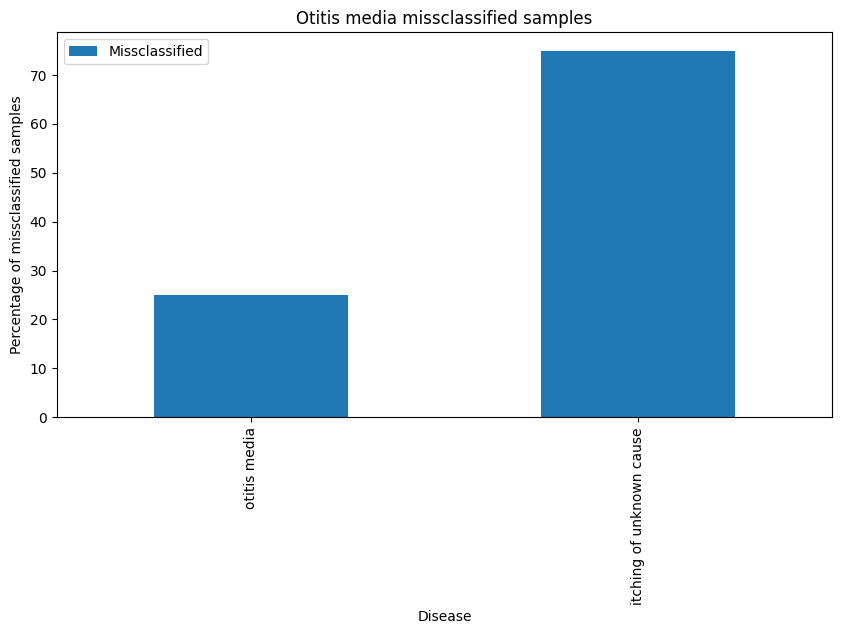
\includegraphics[width=\columnwidth]{otitis_missclassified.png}
	\caption{Percentage of otitis samples misclassified}\label{fig:otitis_missclassified}
\end{figure}
\noindent
\begin{figure}[h]
	\centering
	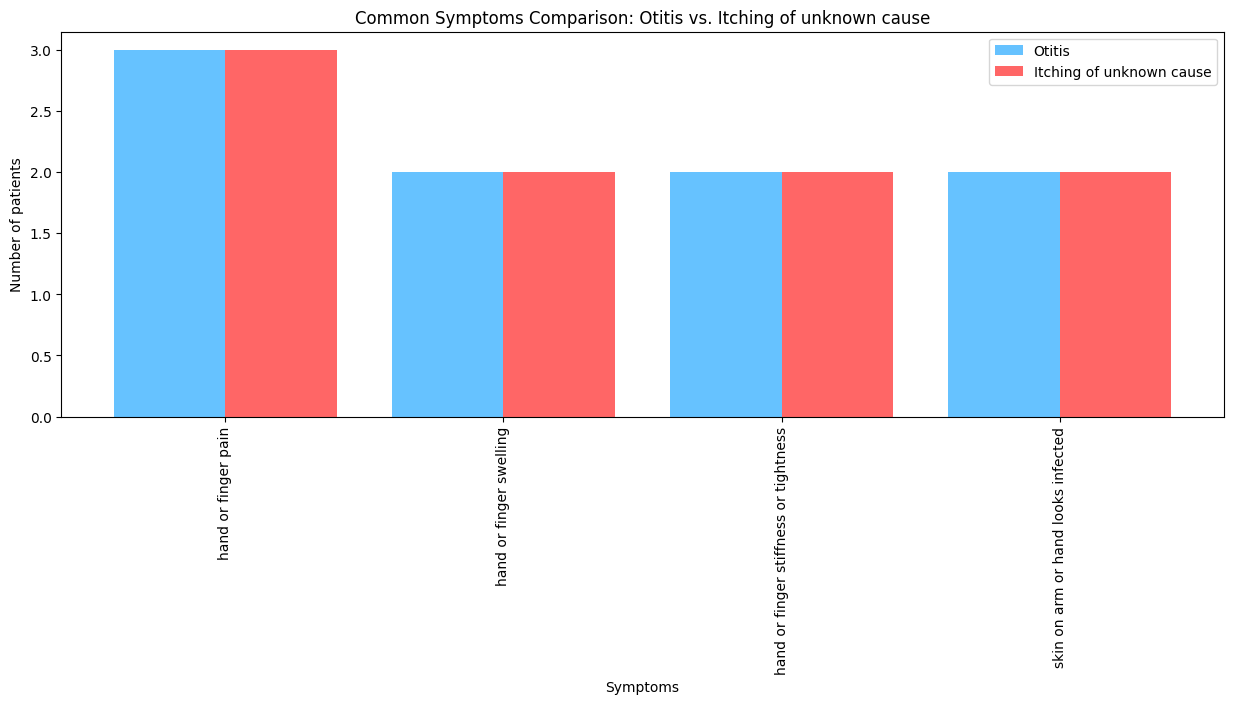
\includegraphics[width=\columnwidth]{otitis_itching.png}
	\caption{number of samples of otitis and itching of unknown cause that have the same symptoms}\label{fig:otitis_itching}
\end{figure}
\noindent

\subsection*{Most impactful symptoms}
Another crucial aspect is to analyze which symptoms are most important for the model.
Since the multiclass version of logistic regression assigns a weight to each symptom for every class,
we have calculated the average absolute value of these weights for each symptom.\\
Figure~\ref{fig:most_important_features} shows the 30 most significant symptoms according to the model.
As can be observed, certain symptoms are more influential. These include both `community size' and `SI index level 2' formats,
such as `sharp chest pain' and `sharp abdominal pain', among others.\\
Furthermore, it is noteworthy that among the three network information types obtained,
none stands out as more important than the others. All three hold significance,
as both `community size' and `SI index level 2' are equally represented among the most important symptoms,
and `community count' is significant for the first two out of three communities.

\begin{figure*}[htbp]
	\centering
	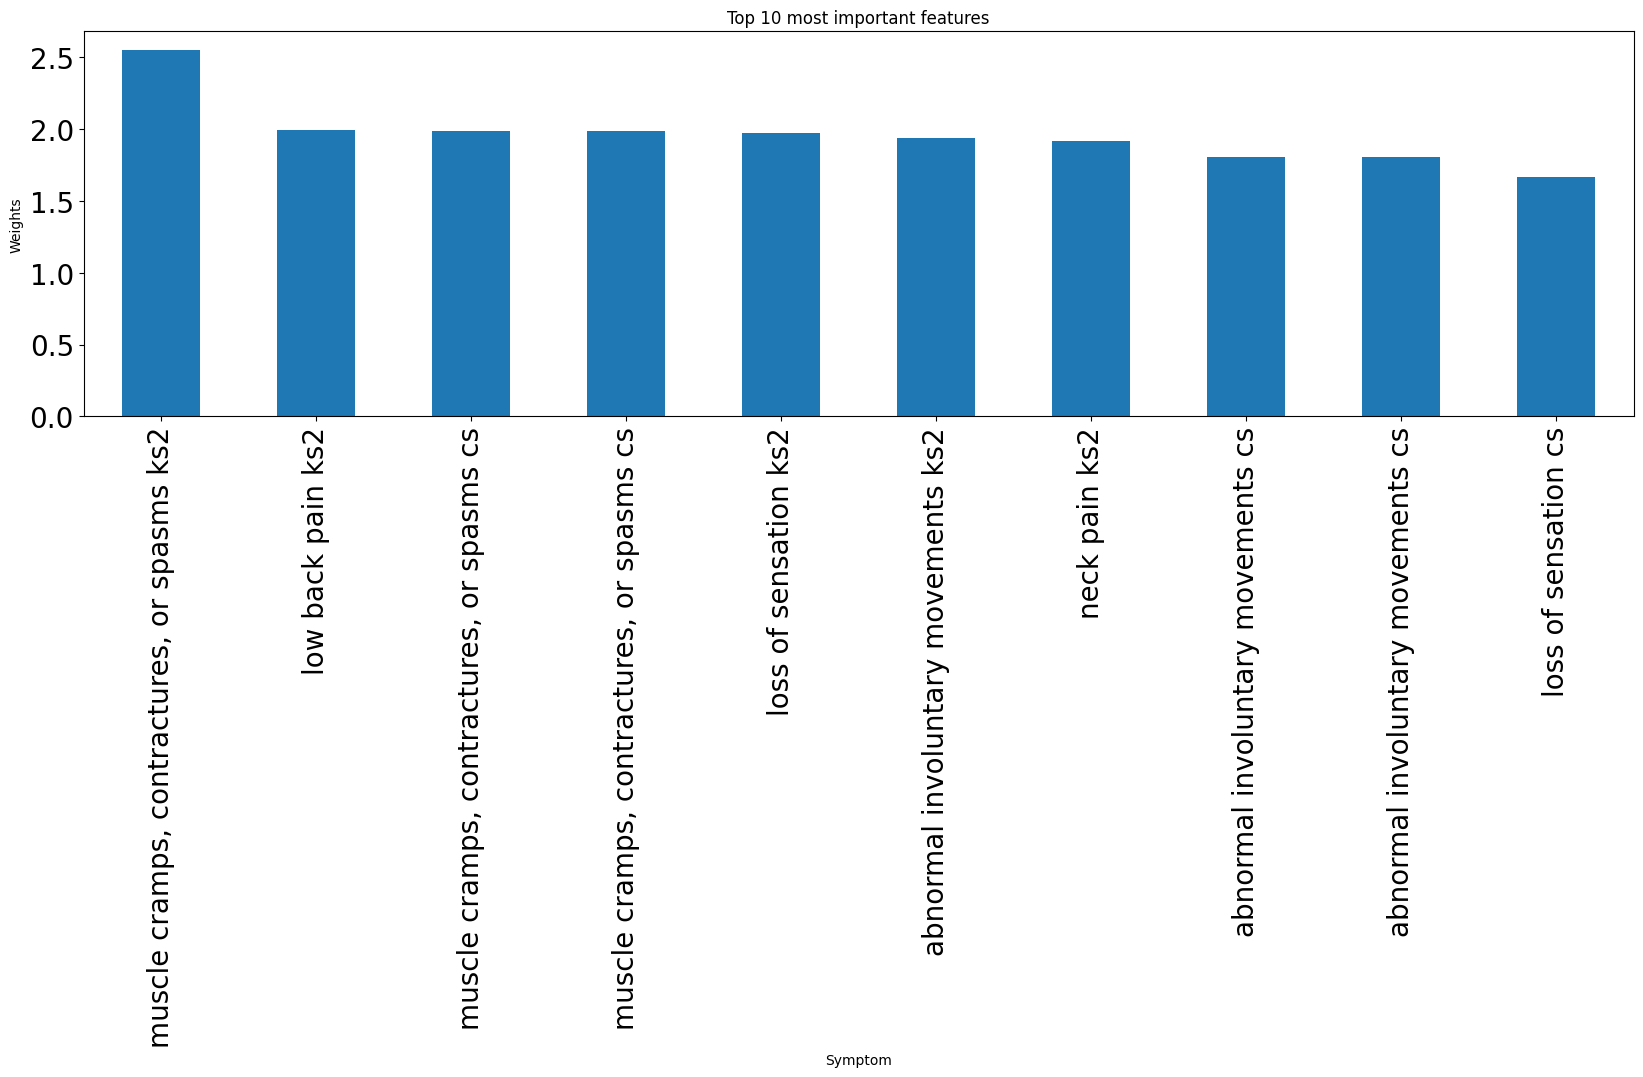
\includegraphics[width=\textwidth]{most_important_features.png}
	\caption{10 most impactful features}\label{fig:most_important_features}
\end{figure*}
\noindent

\subsection{Computational Complexity}
\label{subsec:computational_complexity}
% MATTEO
% - apply the reduction technique based on symptoms importance (L1 and L2 combined in the 4 classes)
% - compare the performance of the reduced model with the original one
% - precision, recall, AUC, accuracy
% - compare the times needed to train the two models
After confirming the presence of some symptoms that are more impactful than others,
we applied a reduction technique based on their importance, leveraging the division
into four classes based on the L1 and L2 Symptom Influence indexes (SI).
The first test was to divide the data into four balanced classes, containing 25\% of the features each.
As shown by Figure~\ref{fig:class_wise_accuracies}, the most impactful set of
features was the one corresponding to the class with both high SI L1 and L2.
This feature class was the one performing better, with only a few classes that were consistently mispredicted.
The worst one was the low-low class, which had a class-wise accuracy of less than 20\% for most of the disease classes.

\begin{figure}[H]
	\centering
	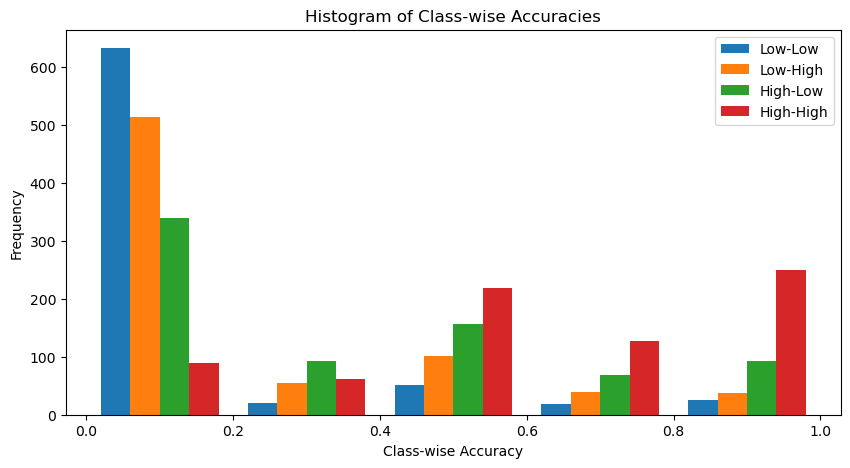
\includegraphics[width=\columnwidth]{class_wise_accuracies.png}
	\caption{Histogram of the class accuracy for each feature group, based on SI L1 and L2.}\label{fig:class_wise_accuracies}
\end{figure}

\noindent
Even then, the high-high class by itself would not be a sufficiently good set of features to make predictions,
so it was used as a baseline to expand the feature set, retaining increasingly more features.
As it can be seen from Figure~\ref{fig:accuracy_vs_features_retained}, the model performance is quite good even when using only
a limited amount of features, reaching around 80\% test accuracy when using half of the features, which corresponds to a
reduction of 10\% of the accuracy of the complete model, giving up half the data.
This is a good trade-off, but the accuracy is valuable, so we decided to give up at most 1\% accuracy,
which in this case corresponds to a reduction of the features by almost 30\%.

\begin{figure}[H]
	\centering
	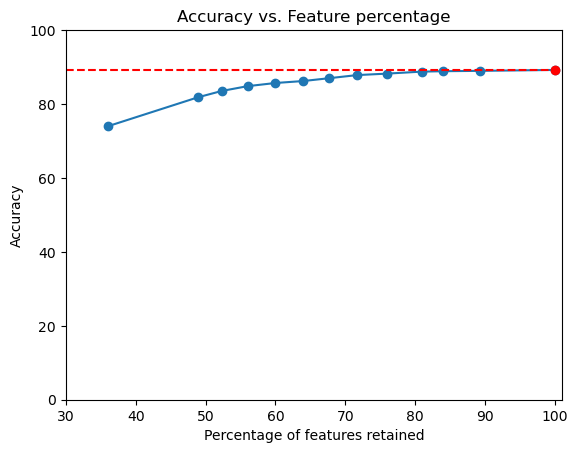
\includegraphics[width=\columnwidth]{accuuracy_vs_features_retained.png}
	\caption{Comparison between the reduction in features against the reduction on the test accuracy.}\label{fig:accuracy_vs_features_retained}
\end{figure}

\noindent
To assess how the reduction of the complexity of the model impacts the training,
we repeated the training phase on the whole balanced dataset, recording the difference in time between the two models.
In the end, the experimental results showed a reduction in training time of 9.39\% caused by a reduction of the training features of 27.87\%.
The relative time reduction is lower in comparison to the whole model, but it shows promising results that
could possibly be even more impactful when dealing with more complex models.

\begin{figure}[H]
	\centering
	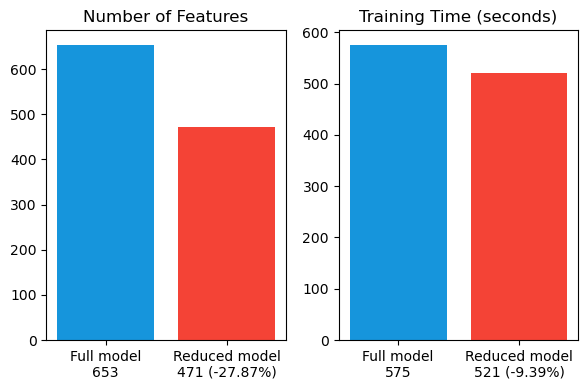
\includegraphics[width=\columnwidth]{features_vs_time.png}
	\caption{Visual rendition of the training time reduction compared to the features.}\label{fig:features_vs_time}
\end{figure}

\noindent
Given the reduction of the features of almost 30\%, the accuracy went down by around a percent and a half,
but to really assess the quality of the reduced model, we cannot rely only on the test accuracy.
Other metrics were employed for the evaluation, which were the precision, recall, and AUC of the ROC.
As depicted by Figure~\ref{fig:precision_recall_auc},
the data showed a similar difference in these metrics, with the exeption of the AUC being almost identical.
This helped us understand that the reduction on the features didn't cause the model to perform well on just the most frequent classes,
but resulted in a good performance across the whole data.

\begin{figure}[H]
	\centering
	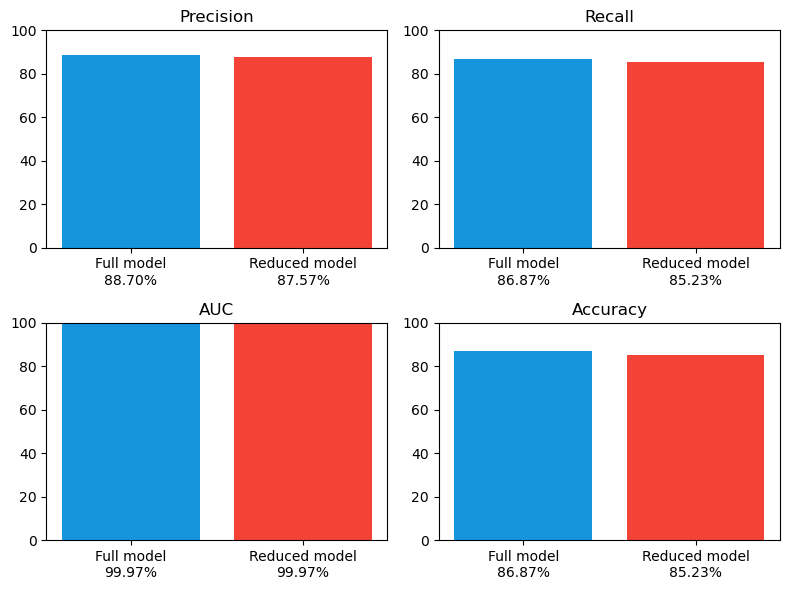
\includegraphics[width=\columnwidth]{precision_recall_auc.png}
	\caption{comparison of various metrics which are useful to asses the relative quality of the reduced model.}\label{fig:precision_recall_auc}
\end{figure}
\noindent

% CRISTIAN
% - 6 Modelli: 3 con solo sintomi, 3 con nuove features
% - - Salvati (joblib) 
% - - Tempo di training

